\begin{exercises} 
  \item Suppose that $T(t)$ represents the temperature of a cup of
    coffee set out in a room, where $T$ is expressed in degrees
    Fahrenheit and $t$ in minutes.  A physical principle known as    Newton's Law of Cooling\index{Newton's Law of Cooling} tells us that 
    $$
    \frac{dT}{dt}= -\frac1{15}T+5.
    $$

\ba
    \item Supposes that $T(0)=105$.  What does the differential
    equation give us for the value of $\ds \frac{dT}{dt}\vert_{T=0}$?  Explain in a
    complete sentence the meaning of these two facts.

    \item Is $T$ increasing or decreasing at $t=0$?

    \item What is the approximate temperature at $t=1$?

    \item On the graph below, make a plot of $dT/dt$ as a function of $T$.
        \begin{center}
          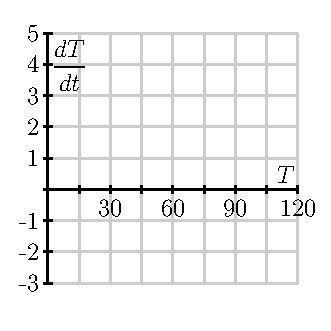
\includegraphics{figures/7_1_exercise_1.eps}
        \end{center}

       \item For which values of $T$ does $T$ increase?  For
        which values of $T$ does $T$ decrease?

        \item What do you think is the temperature of the room?
        Explain your thinking.

        \item Verify that $T(t) = 75 + 30e^{-t/15}$ is the
        solution to the differential equation with initial value $T(0)
        = 105$.  What happens to this solution after a long time?
  \ea
  
  \item Suppose that the population of a particular species is
    described by the function $P(t)$, where $P$ is expressed in
    millions.  Suppose further that the population's rate of change is
    governed by the differential equation 
    $$\frac{dP}{dt} = f(P)
    $$
    where $f(P)$ is the function graphed below.

    \begin{center}
      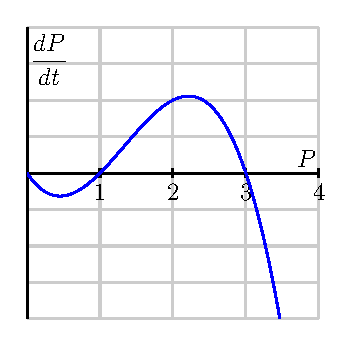
\includegraphics{figures/7_1_threshold.eps}
    \end{center}

\ba
    \item For which values of the population $P$ does the population
      increase?

      \item For which values of the population $P$ does the population
      decrease? 

      \item  If $P(0) = 3$, how will the population change in time?

     \item  If the initial population satisfies $0<P(0)<1$, what will
      happen to the population after a very long time?

      \item  If the initial population satisfies $1<P(0)<3$, what will
      happen to the population after a very long time?

      \item If the initial population satisfies $3<P(0)$, what will
      happen to the population after a very long time?

      \item  This model for a population's growth is sometimes called
      ``growth with a threshold.''  Explain why this is an appropriate
      name.  

\ea

  \item In this problem, we test further what it means for a function to be a solution to a given differential equation.
  \ba
  	\item Consider the differential equation
      $$
      \frac{dy}{dt} = y - t.
      $$
      Determine whether the following functions are solutions to the given differential equation.

      \begin{itemize}
 	\item[(i)] $y(t) = t + 1 + 2e^t$
	\item[(ii)] $y(t) = t + 1$
	\item[(iii)] $y(t) = t + 2$
       \end{itemize}

	\item   When you weigh bananas in a scale at the grocery store, the
      height $h$ of the bananas is described by the differential
      equation
      $$
      \frac{d^2h}{dt^2} = -kh
      $$
      where $k$ is the {\em spring constant}, a constant that depends
      on the properties of the spring in the scale.  After you put the
      bananas in the scale, you (cleverly) observe that the height of the bananas
      is given by $h(t) = 4\sin(3t)$.  What is the value of the spring
      constant? 
    \ea
        
\end{exercises}
\afterexercises
